\section{Pendahuluan}
\subsection{Latar Belakang}
Perkembangan teknologi informasi yang pesat telah mendorong kebutuhan akan jaringan komputer yang handal, efisien, dan aman. Dalam sistem jaringan komputer, proses komunikasi antar perangkat tidak dapat berjalan tanpa adanya aturan atau mekanisme yang jelas. Oleh karena itu, pemahaman terhadap protokol jaringan menjadi hal yang sangat penting, karena protokol inilah yang mengatur bagaimana data dikirim, diterima, dan diproses antar perangkat dalam jaringan. Salah satu protokol inti yang digunakan secara luas dalam jaringan komputer modern adalah TCP/IP, yang menjadi dasar dari komunikasi di internet maupun jaringan lokal. Di dalam sistem TCP/IP, setiap perangkat yang terhubung memerlukan sebuah alamat unik yang disebut IP Address. IP address berfungsi sebagai identitas perangkat agar dapat saling berkomunikasi dalam jaringan. Versi IP yang paling umum digunakan saat ini adalah IPv4, yang menggunakan alamat 32-bit dan mampu menghasilkan lebih dari empat miliar alamat unik. Pemahaman terhadap struktur dan klasifikasi IPv4 sangat penting untuk mengelola dan mengkonfigurasi jaringan, termasuk dalam proses subnetting dan pengalokasian alamat. Selain aspek logis dari jaringan, pemahaman terhadap konektivitas fisik melalui kabel LAN juga menjadi hal yang fundamental. LAN (Local Area Network) memungkinkan koneksi antar perangkat dalam satu area terbatas seperti ruang laboratorium atau kantor. Media koneksi yang digunakan umumnya berupa kabel UTP dengan konektor RJ-45 yang dihubungkan ke perangkat seperti switch dan router. Dengan koneksi LAN kabel, praktikum dapat dilakukan untuk mengamati secara langsung bagaimana perangkat saling terhubung, bagaimana IP address dikonfigurasi, serta bagaimana data dikirim melalui jaringan berdasarkan protokol yang digunakan. Oleh karena itu, praktikum ini bertujuan untuk memberikan pemahaman teoritis sekaligus pengalaman praktis dalam membangun dan mengelola jaringan komputer sederhana, mulai dari aspek pengalamatan IP, konfigurasi IPv4, hingga pemasangan dan pengujian konektivitas menggunakan kabel LAN.


\subsection{Dasar Teori}
Dalam dunia jaringan komputer, protokol jaringan merupakan fondasi utama yang memungkinkan komunikasi antar perangkat dapat terjadi secara efektif, aman, dan terstruktur. Protokol adalah sekumpulan aturan atau standar yang menentukan bagaimana data dipaketkan, dikirim, diterima, dan diinterpretasikan di dalam jaringan. Protokol jaringan yang paling umum digunakan adalah TCP/IP (Transmission Control Protocol/Internet Protocol), yang menjadi dasar dari komunikasi di internet. TCP menjamin keandalan dan urutan transmisi data, sedangkan IP bertugas mengatur pengalamatan dan pengiriman paket antar host. Salah satu komponen penting dalam sistem ini adalah IP Address, yaitu alamat unik yang digunakan oleh setiap perangkat dalam jaringan untuk mengidentifikasi dirinya dan memungkinkan pertukaran data dengan perangkat lain. IP address ibarat alamat rumah bagi perangkat digital, yang memungkinkan data dikirim dan diterima ke tujuan yang tepat. IP address terdiri dari dua versi utama, yaitu IPv4 dan IPv6. Namun, IPv4 (Internet Protocol version 4) masih menjadi versi yang paling banyak digunakan hingga saat ini. IPv4 menggunakan sistem pengalamatan 32-bit yang menghasilkan sekitar 4,3 miliar alamat unik, yang ditulis dalam format desimal dengan empat oktet, seperti 192.168.0.1. Keterbatasan jumlah alamat ini menjadi alasan dikembangkannya IPv6 yang memiliki jangkauan lebih luas. IPv4 juga mendukung teknik seperti subnetting untuk membagi jaringan menjadi segmen-segmen kecil serta NAT (Network Address Translation) untuk menghemat penggunaan alamat IP publik. Untuk menghubungkan perangkat secara fisik dalam satu jaringan lokal, digunakan konektivitas kabel LAN (Local Area Network). LAN adalah jaringan berskala kecil hingga menengah yang biasanya digunakan di rumah, sekolah, kantor, atau gedung. Media transmisi yang umum digunakan pada konektivitas kabel LAN adalah kabel twisted pair seperti UTP (Unshielded Twisted Pair) kategori 5e atau 6, dengan konektor standar RJ-45. Kabel ini menghubungkan perangkat-perangkat seperti komputer, printer, switch, dan router sehingga dapat saling bertukar data dalam satu jaringan. Koneksi kabel LAN menawarkan kecepatan tinggi, stabilitas sinyal, serta latensi rendah, yang menjadikannya pilihan ideal untuk kebutuhan yang menuntut performa tinggi seperti game online, transfer data besar, atau aplikasi industri. Dalam pengoperasiannya, konektivitas LAN kabel sangat bergantung pada pengaturan IP address dan konfigurasi protokol jaringan agar seluruh perangkat dapat saling berkomunikasi dengan lancar dan efisien.

%===========================================================%
\section{Tugas Pendahuluan}
Bagian ini berisi jawaban dari tugas pendahuluan yang telah anda kerjakan, beserta penjelasan dari jawaban tersebut
\begin{enumerate}
	\item Tentukan Rentang IP address dan prefix (CIDR) yang sesuai untuk masing-masing departemen dan total subnet yang diperlukan dan IP network untuk masing-masing.
	\begin{table}[H]
	\centering
	\caption{Rentang IP Address dan Prefix untuk Masing-Masing Departemen}
	\small
	\begin{tabular}{|p{3cm}|p{2.5cm}|p{2cm}|p{4cm}| }
	\hline
	\textbf{Departemen}     & \textbf{IP Network} & \textbf{Prefix (CIDR)} & \textbf{Rentang IP Address}     \\ \hline
	Produksi     & 192.168.1.0         & /26                    & 192.168.1.0 - 192.168.1.63      \\ \hline
	Administrasi & 192.168.4.0         & /27                    & 192.168.4.0 - 192.168.4.31      \\ \hline
	Keuangan     & 192.168.4.32        & /28                    & 192.168.4.32 - 192.168.4.47     \\ \hline
	R\&D         & 192.168.0.0         & /25                    & 192.168.0.0 - 192.168.0.127     \\ \hline
	\end{tabular}
	\label{tab:ip_address}
	\end{table}
	Total subnet = 8.
	
	\item Gambarkan topologi sederhana yang menunjukkan bagaimana router akan menghubungkan semua subnet.
	\begin{figure}[H]
		\centering
		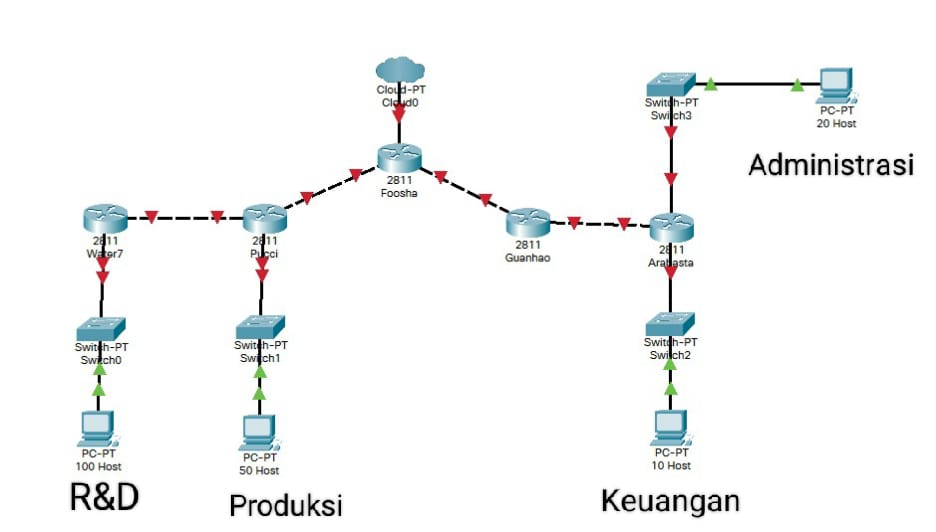
\includegraphics[width=0.8\textwidth]{P1/img/image.png}
		\caption{Topologi Jaringan}
		\label{fig:topologi_sederhana}
	\end{figure}
	
	\item Tabel routing statik pada masing-masing router untuk menjamin konektivitas antar subnet.
	\begin{table}[H]
	\centering
	\caption{Tabel Routing Statis Tiap Router}
	\small
	\begin{tabular}{|p{2cm}|p{4cm}|p{5cm}|}
	\hline
	\textbf{Router} & \textbf{Jaringan Tujuan (Destination Network)} & \textbf{Next Hop} \\ \hline
	Water7 & 192.168.4.0/27, 192.168.4.32/28, 192.168.0.0/25 & 192.168.1.1 \\ \hline
	Plaza & 192.168.1.0/26, 192.168.4.32/28, 192.168.0.0/25 & 192.168.4.1 \\ \hline
	Foosha & 192.168.1.0/26, 192.168.4.0/27, 192.168.4.32/28, 192.168.0.0/25 & Sudah terhubung langsung (core router) \\ \hline
	Guanhao & 192.168.1.0/26, 192.168.4.0/27, 192.168.4.32/28 & 192.168.10.1 \\ \hline
	Arabasta & 192.168.1.0/26, 192.168.4.0/27, 192.168.4.32/28 & 192.168.10.2 \\ \hline
	\end{tabular}
	\label{tab:routing_table}
	\end{table}

	\item Berdasarkan topologi jaringan yang telah dibuat, jenis routing yang paling cocok untuk perusahaan ini adalah kombinasi antara \textbf{Static Routing} dan \textbf{Classless Inter-Domain Routing (CIDR)}.

	\textbf{Justifikasi:}
	\begin{itemize}
		\item \textbf{Topologi Sederhana dan Stabil:} Jaringan terdiri dari sedikit router dan subnet. Static routing mudah dikonfigurasi, cukup aman, dan tidak memerlukan overhead tinggi.
		
		\item \textbf{Penggunaan CIDR:} Alokasi IP address menggunakan subnet yang efisien seperti /25, /26, /27, dan /28. Ini memungkinkan penghematan IP address dan fleksibilitas dalam manajemen jaringan.
		
		\item \textbf{Dynamic Routing Tidak Diperlukan:} Protokol seperti OSPF atau EIGRP akan menambah kompleksitas dan penggunaan resource. Karena topologi tidak berubah-ubah, static routing lebih ideal.
	\end{itemize}

	\textbf{Kesimpulan:} Static routing + CIDR adalah pilihan optimal untuk jaringan ini karena efisien, hemat sumber daya, dan sesuai dengan kebutuhan organisasi.
\end{enumerate}

